\chapter{Developing Unplagged}\label{chap:developingUnplagged}

Coming from the \nameref{chap:systemRequirements} here we have yet another set of requirements, before we can
start with the actual description of the used technologies within the system. This time it's 
about what we believe will be helpful or sometimes even necessary prerequisites. 

First of all, the programming languages mostly used in Unplagged are PHP and JavaScript, both of which in conjuction
with a framework. Teaching programming languages is, as you probably can imagine, well beyond the scope of this document,
but we will at least try to cover the most important concepts of the frameworks as they occur. 

The used frameworks are 
\href{http://jquery.com/}{jQuery} for Javascript and \href{http://framework.zend.com/docs/overview}{ZEND} for PHP 
respectively. jQuery is kind of the industry standard for unobtrusive scripting with about 50\% 
of the Top 10.000 websites using it according to \citet{Trends} and the Zend framework is also well established and
brings a lot of features, that are useful to this project.

For most of the other topics, we will give you some (hopefully) helpful resources on the way, if it isn't covered 
thoroughly by us. But just to let you
know, here is a list of the buzzwords, err technologies that will be mentioned:

\begin{itemize}
\item HTML5 and CSS3
\item Continuous Integration
\item Responsive Webdesign
\item Progressive Enhancement
\item Git, Netbeans, Redmine
\item Tesseract, Imagemagick, Simtext
\end{itemize}

As said before, the system is developed, so that it should work on multiple platforms. 
This makes it sometimes difficult to describe certain installation processes in a way that would work for everybody. As
it's often most problematic, to get some Linux software running on Windows, we will mostly concentrate on the way those
things are done on this platform and give the instructions for other operating systems as an aside if necessary.

\section{Development Environment}

The following section will mostly focus on the way you can get a development version of unplagged up and running on your 
system.

\subsection{Git}
The source code and files of all parts of the Unplagged project are managed through Git, 
with the repository hosted at \href{https://github.com}{Github}. 
Git is a distributed version control system, that exists since 2005 and gained more and more 
track in recent years. Many developers prefer it over other version control systems, because it is much easier 
to create different branches and merge them again or simply initalize local repositories. This
made it also interesting for us to use it for Unplagged. % citation?

However, none of the team members had ever used 
Git before in a bigger context so it was a challenge to get a common workflow running on all the systems. But we took it, 
to explore all the 
features Git offers.

% This feels weird, because the description afterwards is actually nearly the same as in the video, so why show it?
% I think we should strike this point

%If you have experience with more classical central version control systems, but didn't use git before, it would probably 
%be a good idea, to watch this 8 minutes Git introduction as a starting point, because it compares the Git worfklow to Subversions:

%\begin{itemize}
%\item \url{http://www.youtube.com/watch?v=RDGzF2M-zlo}
%\end{itemize}

\subsubsection{Installing Git Bash}

First of all let's find out, how to install the Git console application, called Git Bash. 
Unfortunately all the GUIs we were evaluating didn't work consistently, so we decided to use it from the command line 
only. 
A very good instruction on how to install the Git Bash can be found on the website of the github project:

\begin{description}
\item[Windows:] \url{http://help.github.com/win-set-up-git/}
\item[Linux:] \url{http://help.github.com/linux-set-up-git/}
\item[Mac OS X:] \url{http://help.github.com/mac-set-up-git/}
\end{description}

\subsubsection{Getting the source code of the unplagged project}
Now it is time to get the project source code on your machine. As said before, the whole unplagged project is hosted 
on 
github, so if you want to be able to contribute source code later on, you first need to create an account there:

\begin{itemize} 
\item \url{https://github.com}
\end{itemize}

This isn't necessary, if you simply want to look into the source code, which can be accessed via the repository URL:

\begin{itemize}
\item \url{https://github.com/benoertel/unplagged}
\end{itemize}

If you haven't been granted write access to the above mentioned repository by a project member (which is very likely 
when
you are reading this document for the first time), you will need to do a fork
of the Unplagged project right at github, like described in:

\begin{itemize}
\item \url{http://help.github.com/fork-a-repo/}
\end{itemize}

After this, the following steps are mostly the same for everybody, with the distinction of the project URIs, 
which should be the one of your newly created fork.

Open up the Git Bash and switch to the directory where you want the project to be 
located and clone the repository as you can see in listing \ref{list:cloning}. 

\begin{lstlisting}[caption=Cloning a repository, label=list:cloning]
cd ?Sites/unplagged.local?
git clone ?https://\textbf{<username>}@github.com/benoertel/unplagged.git?
\end{lstlisting}

After this you should have a local copy of all the repository data in the specified directory.

\subsubsection{The most important git commands}

You are now ready to use Git! Here are some more instructions on the most important commands and how to properly 
use it. 
However, if the given instructions in this manual are not enough, feel free to checkout the whole Git manual on: 

\begin{itemize}
\item \url{http://schacon.github.com/git/user-manual.html}
\end{itemize}

The Unplagged project consists of several branches, which are used to develop and store code independently of the other 
developers. Once a new feature is done, it is merged into the master branch. The master branch usually includes only 
fully tested and deployable source code. 

As a new developer, it is important to create an own branch before doing anything else and switch to it.

\begin{lstlisting}[caption=Creating branches]
git branch mynewfeature
git checkout mynewfeature
\end{lstlisting}

Now anything in the repository can be changed. At any point changes can be versioned in the repository by using the 
\texttt{git commit} 
command. If new files were created, \texttt{git add} has to be executed as well.

\begin{lstlisting}[caption=Adding all new files and commiting]
git add .
git commit -m "A message that describes the changes."
\end{lstlisting}

When the feature is fully working and approved, it has to be merged back to the master branch, in order to get 
deployed to the staging environment. To do this, the master branch has to be checked out, updated with \texttt{git pull} 
and then all changes have to be merged from the new feature into the master branch. The feature branch can then be
removed.

\begin{lstlisting}[caption=Merging branch into master]
git checkout master
git pull
git merge mynewfeature
git branch -d mynewfeature
\end{lstlisting}

In comparison to Subversion for example, Git has one more step to really write back to the remote source repository. 
After a \texttt{git commit}, a \texttt{git push} has to be executed, each push can include multiple commits.

\begin{lstlisting}[caption=Pushing to the server]
git push origin master
\end{lstlisting}

This is nearly it, the changes to the repository have been pushed to the master branch. The only thing, that probably 
has to be done
now, is to open up a pull request on github, if you developed on your own fork of the project. This means, that you 
are
asking the project members who have access to the \enquote{real} Unplagged github account, to integrate your changes 
into the actual project
sources. A nice description of how this process is done can be found at github again:

\begin{itemize}
\item \url{http://help.github.com/send-pull-requests/}
\end{itemize}

\subsubsection{Handling conflicts in merging process}

It is possible, if two developers were working on the same part of a file, that a conflict is found during the merge. 
Such 
a conflict could look like this:

\begin{lstlisting}[caption=Merge conflict, keywordstyle=\color{black}]
CONFLICT (content): Merge conflict in readme.txt

To https://github.com/benoertel/unplagged.git
 ! [rejected]        master -> master (non-fast-forward)
error: failed to push some refs to 'https://github.com/benoertel/unplagged.git'
To prevent you from losing history, non-fast-forward updates were rejected
Merge the remote changes (e.g. 'git pull') before pushing again.  See the
'Note about fast-forwards' section of 'git push --help' for details.

# Unmerged paths:
#   (use "git add/rm <file>..." as appropriate to mark resolution)
#
#    both modified:      readme.txt
#
\end{lstlisting}

To resolve the issues, open the files listed in the error message, in this case \textit{readme.txt} and decide how 
the correct 
version should look like, by removing or changingn all the \enquote{< < < < < < <  HEAD} and 
\enquote{> > > > > > > b478801d68267ef479acc5ca54544634c52c545c} 
parts accordingly or using a dedicated merge tool, that is able to show you the changes that were made

Here is an example of how this process would work:

\begin{lstlisting}[caption=Conflicted file, keywordstyle=\color{black}]
<<<<<<< HEAD
The goal of this project is the creation of an easy-to-use, web-based
system to document and detect plagiarism in scientific papers.

hello world
=======

The goal of this project is the creation of an easy-to-use, web-based
system to document and detect plagiarism in scientific papers.

>>>>>>> b478801d68267ef479acc5ca54544634c52c545c
Just a change for educational purposes.
\end{lstlisting}

It could look like this after merging:


\begin{lstlisting}[caption=Fixed conflict after merging, keywordstyle=\color{black}]
The goal of this project is the creation of an easy-to-use, web-based
system to document and detect plagiarism in scientific papers.

hello world

Just a change for educational purposes.
\end{lstlisting}

\subsection{Local Deployment}

This subsection will describe how to configure a virtual host properly. A virtual host is a domain that is mapped to 
the local web server. It is assumed that Apache, MySQL and PHP are already running on the machine. If not, here are 
some tutorial to get them all running:

\begin{description}
\item [Windows:] \hfill \\
 \url{http://www.apachefriends.org/de/xampp-windows.html#1098}
\item [Mac OS:] \hfill \\
\url{http://www.djangoapp.com/blog/2011/07/24/installation-of-mysql-server-on-mac-os-x-lion/} \\
\url{http://www.quarkstar.at/index.php/2009/05/18/webserver-aktivieren-und-konfigurieren-in-mac-os-x/}
\end{description}

Most Linux distributions should already have this kind of server stack installed.

The main goal to make the system run, is to create a local domain and add the virtual host from listing \ref{list:vhost} 
to the vhost config. 

In Max~OS~X this can be done via 
the command line: 

\begin{lstlisting}[caption=Mac OS X: Creating virtual host, language=bash]
sudo vi ?\textbf{/private/etc/hosts}?
#add the following line:
"127.0.0.1 unplagged.local"

sudo vi ?\textbf{/private/etc/apache2/extra/httpd-vhosts.conf}?
\end{lstlisting}

On Windows you need to open up your \textit{hosts} file, which is mostly located in \\
\textit{C:\textbackslash WINDOWS\textbackslash system32\textbackslash drivers\textbackslash etc\textbackslash hosts}, 
and add the following line on the bottom:

\begin{lstlisting}[caption=New host declaration]
127.0.0.1 unplagged.?local?
\end{lstlisting}

Now you need to open your apache configuration file 
\textit{C:\textbackslash xampp\textbackslash apache\textbackslash conf\textbackslash httpd.conf} and 
remove the hash symbol(uncomment) from the following line

\begin{lstlisting}[caption=httpd.conf]
#Include conf/extra/httpd-vhosts.conf
\end{lstlisting}

Add the following configuration to the httpd-vhosts.conf file you just included:

\begin{lstlisting}[caption=Apache configuration, label=list:vhost]
<VirtualHost *:80>
  ServerName unplagged.?local?
  DocumentRoot ?\enquote{\textbf{/Users/me/Sites/unplagged.local/public}}? 
  SetEnv APPLICATION_ENV "development" 
  
  <Directory ?\enquote{\textbf{/Users/benjamin/Sites/unplagged.local/public}}>?
    Options +Indexes +FollowSymLinks +ExecCGI
    DirectoryIndex /index.php
    AllowOverride All
    Order allow,deny
    Allow from all
  </Directory>
</VirtualHost>
\end{lstlisting}

You can tryout your new configuration by entering \textit{unplagged.local} in your browser.

\subsection{Netbeans}

\subsubsection{Configuring Tests}

\subsubsection{Documentation}

Unplagged uses \href{http://apigen.org/}{\citet{Apigen}} for the generation of a HTML page of all the source code documentation comments, 
because of it's superior and much more beautiful user interface in comparison to the older 
\href{http://www.phpdoc.org/}{\citet{PHPDocumentor}}.

Sadly the automatic generation is not yet supported by Netbeans, but as it will be soon\citep{Heise2012}, we are
currently only generating this server-side as described in section \ref{sec:continuousIntegration}. 

This section will be enhanced, when the Netbeans user interface becomes available. If you are interested, you could 
install the software for yourself and use it over the command line.

\subsection{Additional Software}

As we currently have no installer or script that checks for installed software, you still have to install some
additional dependencies to make some parts of the system work. Those are mainly command line tools that we use
for the optical character recognition or text comparison.

Most of the times the software wouldn't break completely if those dependencies were not installed, but some parts 
would silently fail, which is of course one of the more annoying problems to debug.

\subsubsection{Tesseract}

Tesseract is an open source OCR\footnote{Optical character recognition} software, that is currently used to \enquote{figure out}
texts from scanned images a user can upload. 

The big idea is to build the system in a way that enables users to
plugin their favourite OCR system, but to have one default system that produces satisfying results in Tesseract.

You can download the latest installation files from:

\begin{itemize}
\item \url{http://code.google.com/p/tesseract-ocr/downloads/list}
\end{itemize}

After installing Tesseract, the easiest way to make it work with Unplagged, is to put it on your systems execution path,
so that it could be called from the command line in any directoy.

If for some reason you don't want to do this, you can also change the following line in 
\texttt{/application/configs/application.ini} to the path where you installed Tesseract to:

\begin{lstlisting}[caption=Tesseract executable path]
parser.tesseractPath = 'tesseract'
\end{lstlisting}

You should be able to click the \enquote{parse} icon on files now:

\begin{figure}[htbp]
  \centering
    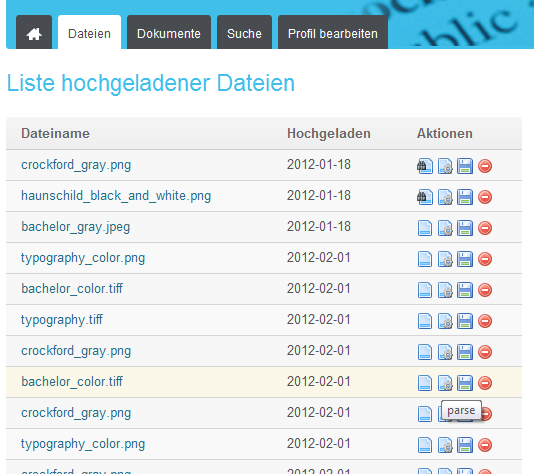
\includegraphics[width=0.9\textwidth]{images/parse-button.png}
  \caption{Parsing Files with Tesseract}
  \label{fig:parseButton}
\end{figure}

\subsubsection{Imagemagick}

Because Tesseract and probably other OCR systems that are provided via a plugin won't work with every image format a 
user decides to upload, we integrated Imagemagick as a tool to convert images from one format to another. To install
it you can simply follow the installation instructions provided here:

\begin{itemize}
\item \url{http://imagemagick.org/script/binary-releases.php}
\end{itemize}

Similar as with Tesseract, you can change the ini directive \texttt{parser.imagemagickPath}, if you chose not to include
the executable in your path.

If you installed it properly, you can try to upload an image file other than \textit{.tiff} and parse it with Tesseract,
which should work now.

\subsubsection{Simtext}

Simtext is a text comparison tool, that is able to output nice data of the differences between texts. In figure 
\ref{fig:simtextOutput} for example, you can see the default side-by-side comparison and in figure \ref{fig:simtextDiff}, 
the output in \textit{diff} format is shown.

\begin{figure}[htbp]
  \centering
    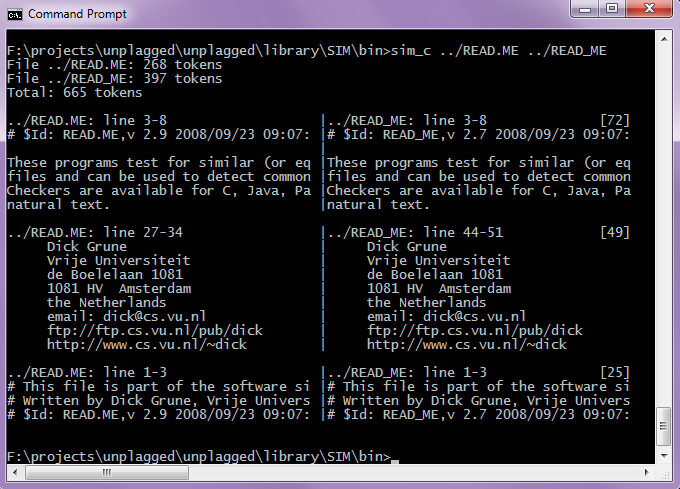
\includegraphics[width=\textwidth]{images/simtext-output.png}
  \caption{Default Simtext output}
  \label{fig:simtextOutput}
\end{figure}

\begin{figure}[htbp]
  \centering
    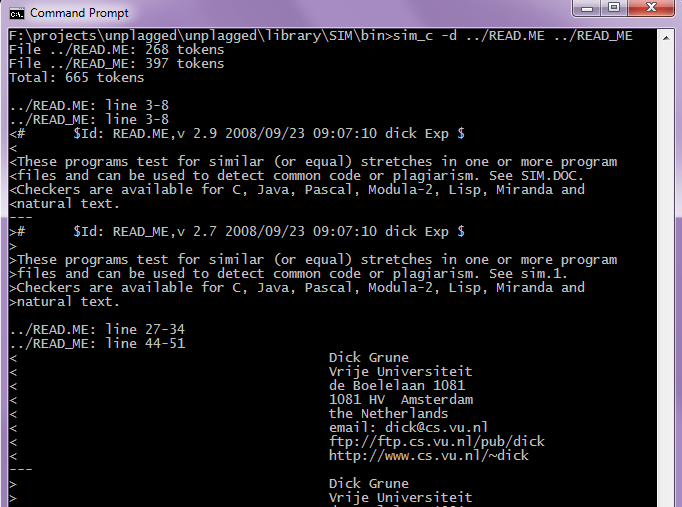
\includegraphics[width=0.8\textwidth]{images/simtext-output-diff.png}
  \caption{Simtext output in diff format}
  \label{fig:simtextDiff}
\end{figure}

Installing Simtext can sadly be a bit tricky, because only the sources and no executables(at least none that worked for us) 
are distributed. We already
provided a Windows 64bit EXE and an executable that runs on our Ubuntu staging environment in \texttt{/library/SIM/bin}, 
but if you use any other environment, you will have to compile the C sources of the system for yourself. The sources can
be found here:

\begin{itemize}
\item \url{http://dickgrune.com/Programs/similarity_tester/}
\end{itemize} 

We assume, that Linux users will be familiar with the installation steps that are described in the readme file. The only
thing that can be easily overlooked there is the necessity to install \textit{Flex} first. Windows
however needs some special treatment to make the compilation work:

\begin{enumerate}
\item Download and install \enquote{Make for Windows} from \url{http://gnuwin32.sourceforge.net/packages/make.htm} and 
\enquote{Flex for Windows} from \url{http://gnuwin32.sourceforge.net/packages/flex.htm}
\item Add the folder of the binaries to the path (should be something like 
\texttt{C:\textbackslash Program Files (x86) \textbackslash GnuWin32\textbackslash bin})
\item Rename \enquote{flex.exe} to \enquote{lex.exe} in the above mentioned directory
\item Unzip and open Simtext directory on the command line and type:
\end{enumerate}
\begin{lstlisting}[caption=Installing and checking simtext, language=bash]
>make
>sim_c --help
>sim_c READ.ME READ_ME
\end{lstlisting}

And again, to make it work you can set the ini directive \texttt{simtext.simtextPath} to the appropriate path or simply
include it in your systems path variable.

\subsection{Continuous Integration}\label{sec:continuousIntegration}

To always have a running version of the latest code, we use an automated workflow, that always deploys everything that 
has been pushed to the Github repository on the Unplagged staging server. The machine this is done with, is a simple 
Ubuntu web server, that is also used for hosting our collaboration tools and the webpage.

\begin{figure}[!h]
  \centering
  \fbox{
    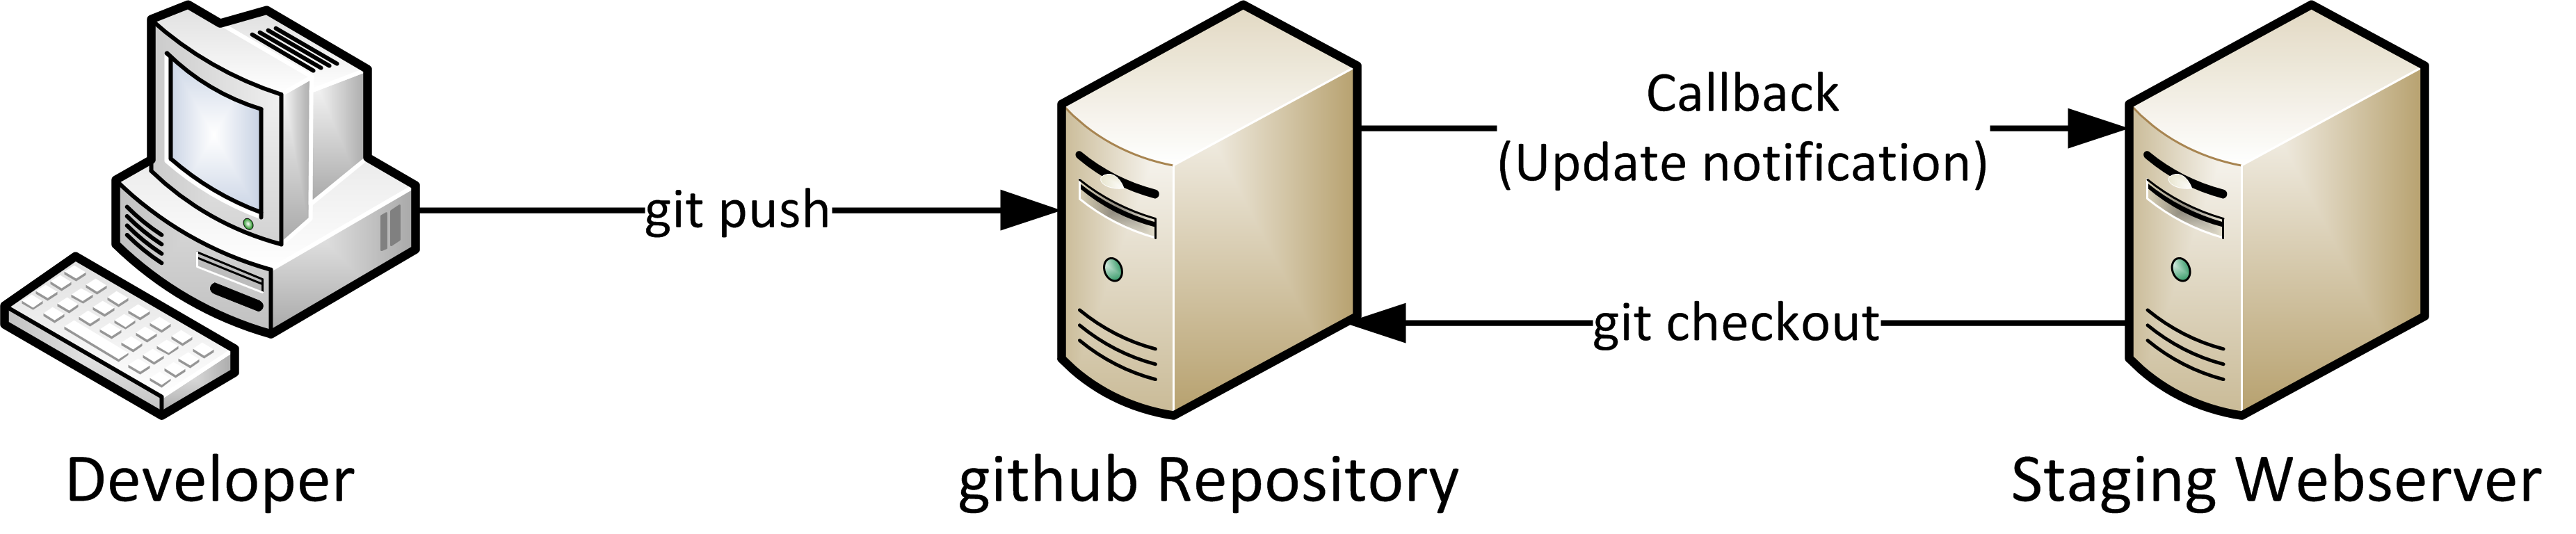
\includegraphics[width=0.97\textwidth]{diagrams/staging-workflow.png}
  }
  \caption{Deployment workflow}
  \label{fig:developmentWorkflow}
\end{figure}

As you can see in figure \ref{fig:developmentWorkflow} the mechanism used for this is a callback, the 
\textit{post-receive hook} of git, 
which github employs to let it's users enter a \textit{post-receive URL} to call a URL after someone has pushed to the
repository. The URL that gets called is located on our staging server and gets answered by a Redmine plugin called 
\enquote{redmine\_github\_hook}, that would
normally only call a checkout on the server-side repository, so that the newest sources can be seen via the Redmine
web frontend. 

\begin{lstlisting}[caption=Changes to redmine\_github\_hook.rb, label=list:redmineGithubHook, language=Ruby]
# Fetches updates from the remote repository
def update_repository(repository)
  command = git_command('fetch origin', repository)
  if exec(command)
    command = git_command("fetch origin '+refs/heads/*:refs/heads/*'", repository)
    exec(command)

    #custom checkout to preview area
    system('sh /usr/local/etc/scripts/buildUnplaggedPreview.sh')?\label{customRubyChange}?
  end
end
\end{lstlisting}

However, we tweaked the source code of this plugin slightly, as you can see on line \ref{customRubyChange}
in listing \ref{list:redmineGithubHook} so that it also calls the below bash script(listing \ref{list:deploymentScript})
to initiate the deployment process.

\lstset{language=bash}
\begin{lstlisting}[caption=Deployment script, language=bash, label=list:deploymentScript]
#!/bin/bash

cd /var/git/unplagged.git/
GIT_WORK_TREE=/var/www/preview.unplagged.com git checkout -f

cd /var/www/preview.unplagged.com
#generate phpdoc
apigen -s application/ -s library/Unplagged/ -d docs/phpdoc --title "Unplagged Documentation" --todo yes

#run database build scripts
cd scripts/build
php initdirectories.php
php doctrine_staging.php

cd /var/www
chown www-data:www-data preview.unplagged.com
\end{lstlisting}

The bash script is then used to do a \enquote{clean checkout}(without hidden \texttt{.git} folders) of the repository and
to run \enquote{Apigen}, an engine to process the PHPDoc comments inside the project.
Those two things can be accessed by the already prepared vHosts on the server:

\begin{itemize}
\item \url{http://preview.unplagged.com/}
\item \url{http://phpdoc.unplagged.com/}
\end{itemize}

If you would like to get access to the preview areas, you need to obtain the password and username from a team member.

\subsubsection{Possible Improvements}

The above described workflow is, as we believe, already on a good way, but it still has a lot of room for improvement. 
First of all, it would
be nice to only let the deployment go through, if the unit tests ran successfully on the server and to have some sort of 
email notification mechanism if this wasn't the case.

Another improvement would also be to have a separation into a staging environment with the newest commits and an 
actual preview environment, that can be deployed to a known stable state/commit of the system in a simple manner.

\section{User Interface / User Experience}

Here we will explain the progress and development of the user interface of Unplagged. As we tried to follow the 
typical project workflow, we first drew a lot of mockups in the beginning, which represented the main features of 
Unplagged. At first the wireframes, or also called mockups were drawn by hand, before we digitalized them. As an example 
the mockups of the 'new case' page are shown below in figure \ref{fig:mNewCaseMockup}. All the other mockups can be found 
in the appendix \ref{appendix:mockups}.

\begin{figure}[htbp]
  \centering
    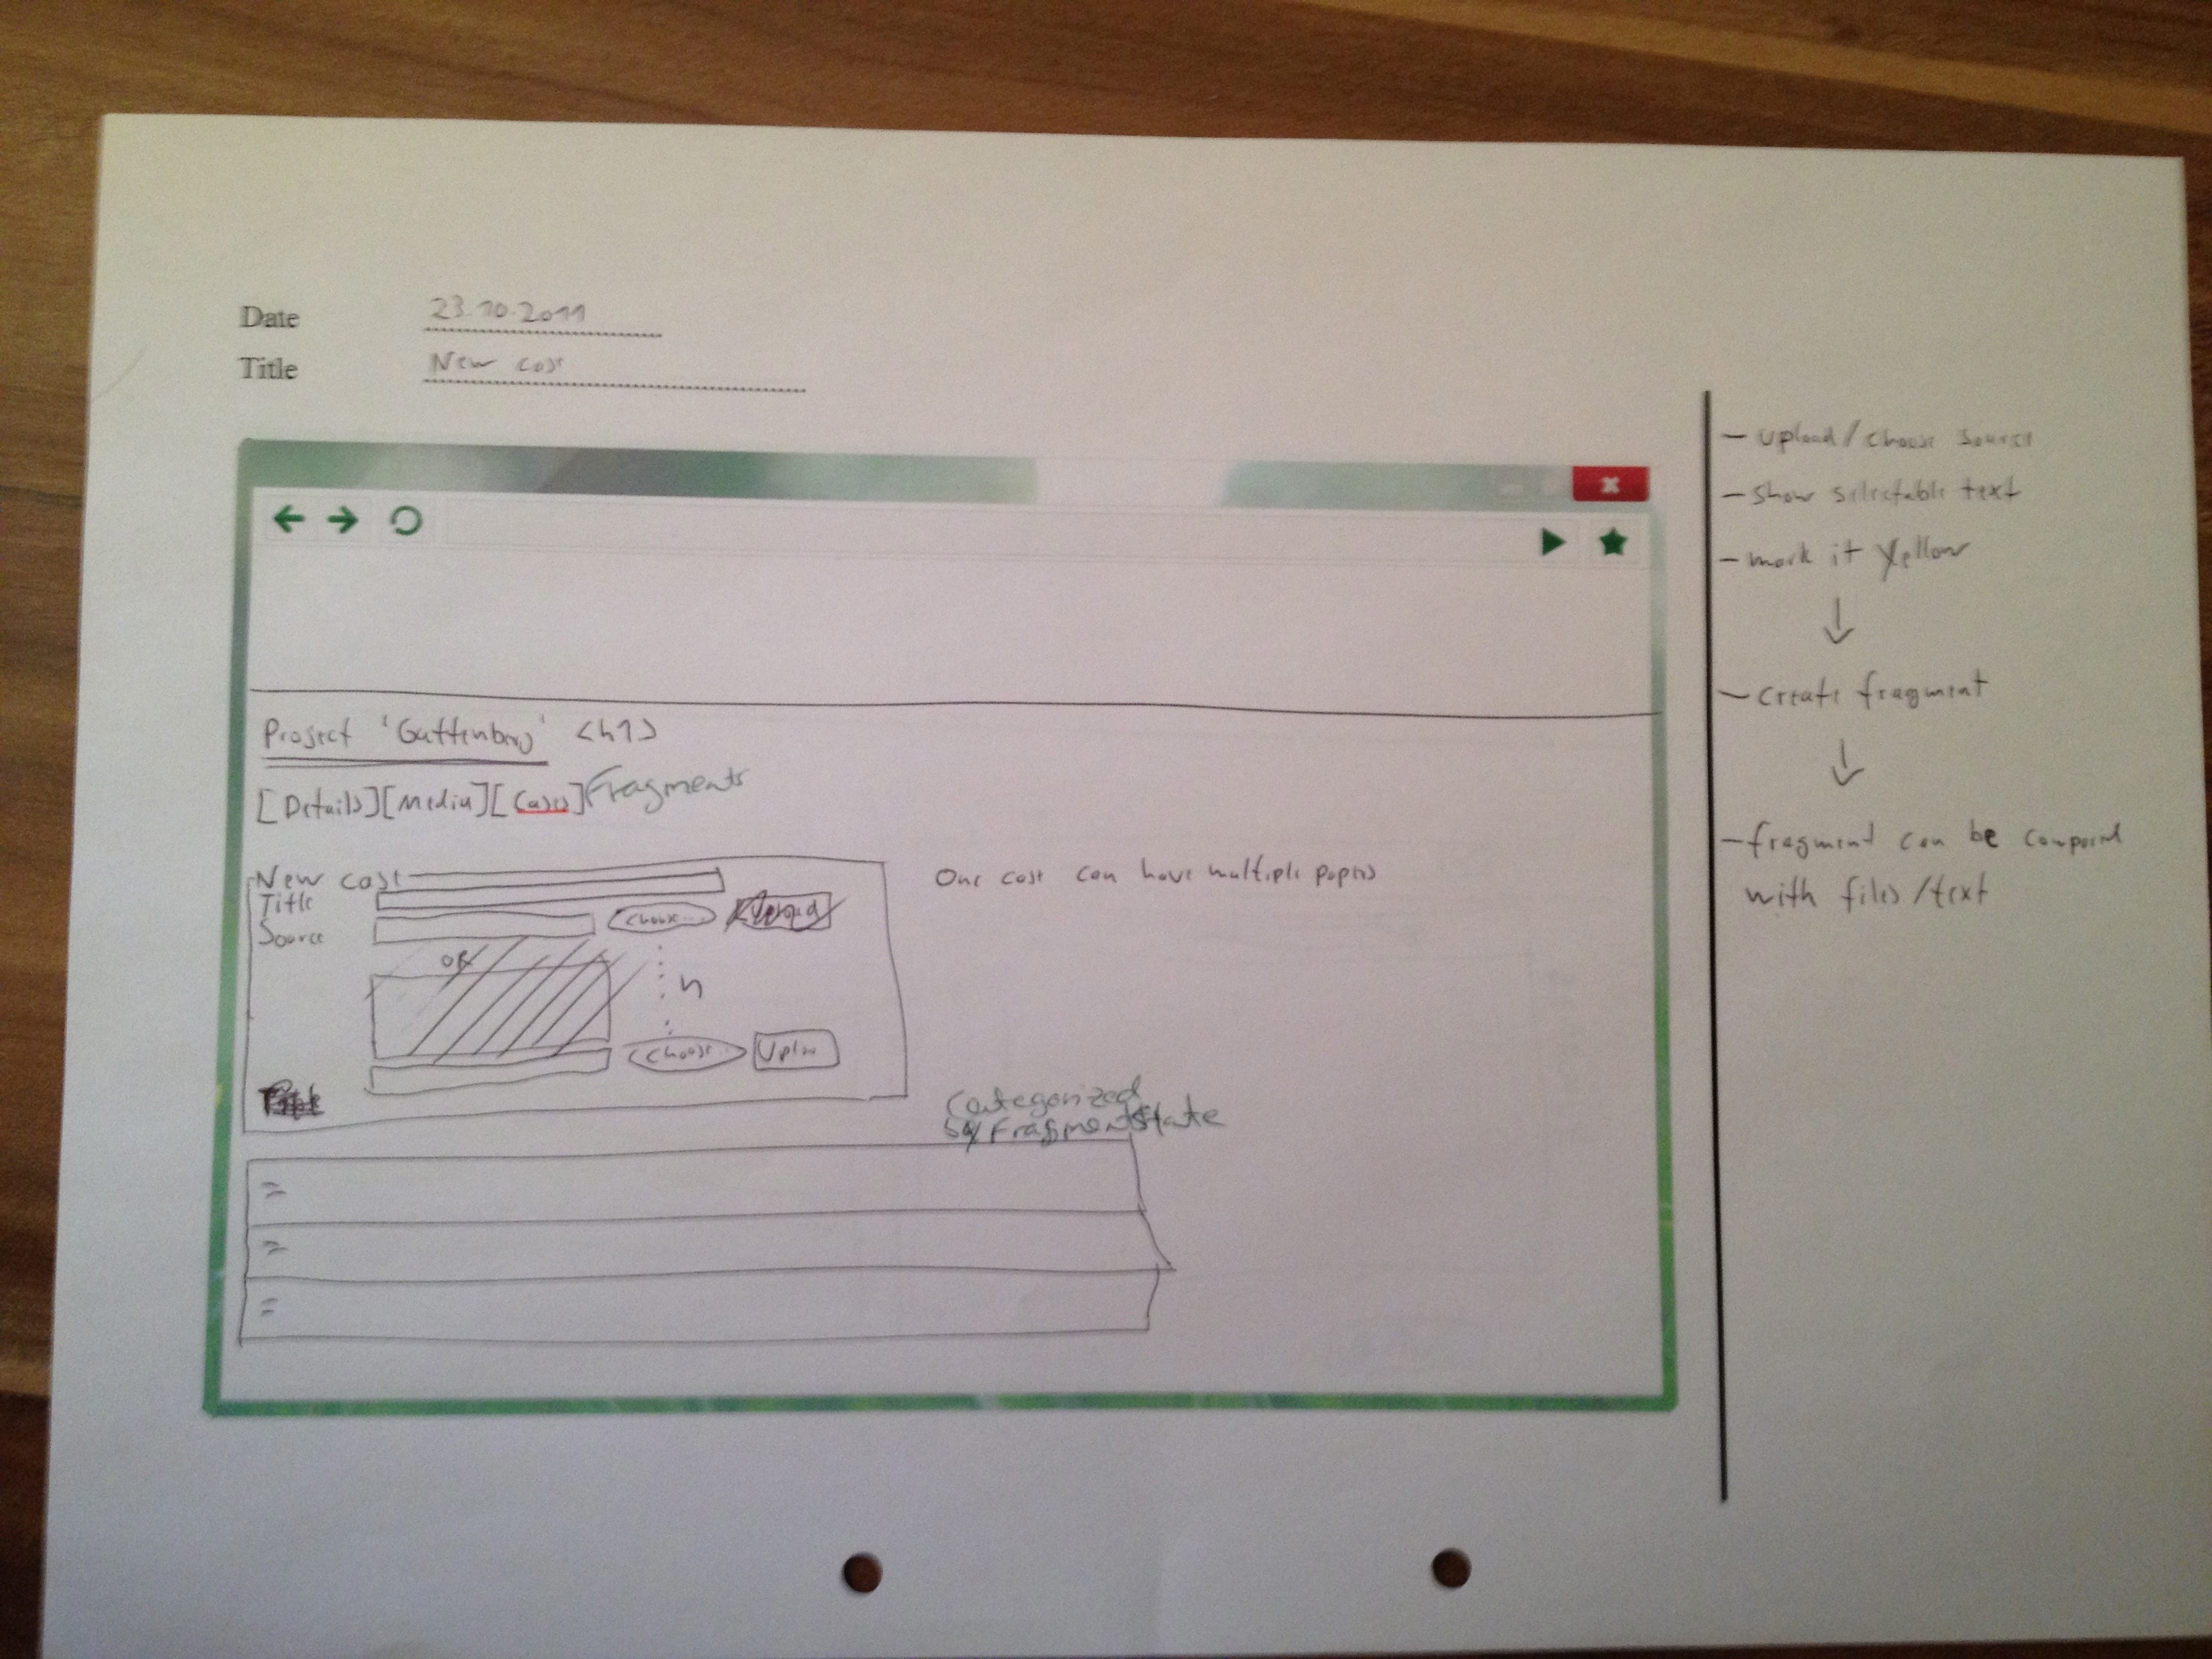
\includegraphics[width=0.97\textwidth]{mockups/m_new_case.jpg}
  \caption{Mockup -- New case -- hand-drawn}
  \label{fig:mNewCaseMockup}
\end{figure}

\begin{figure}[htbp]
  \centering
    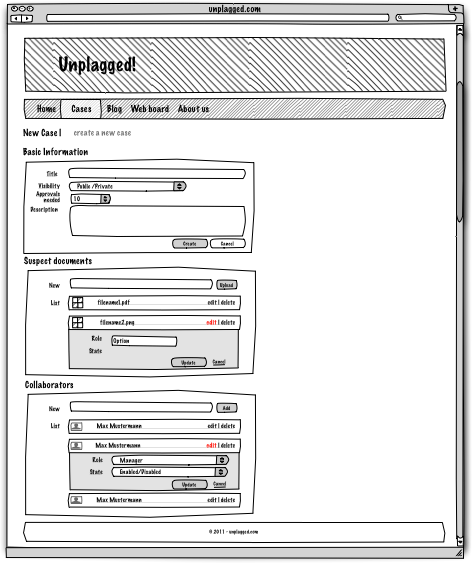
\includegraphics[width=0.97\textwidth , bb = 0 250 490 560,clip]{mockups/1_new_case.png}
  \caption{Mockup -- New case -- digitalized}
  \label{fig:1newCaseMockup}
\end{figure}


After we had a basic idea how the main interface should be structured, we created a first screen in Photoshop. Therefore 
we got several helpful suggestions from the website PremiumPixels: 

\begin{itemize}
\item \url{http://www.premiumpixels.com/}.
\end{itemize}

\begin{figure}[htbp]
  \centering
    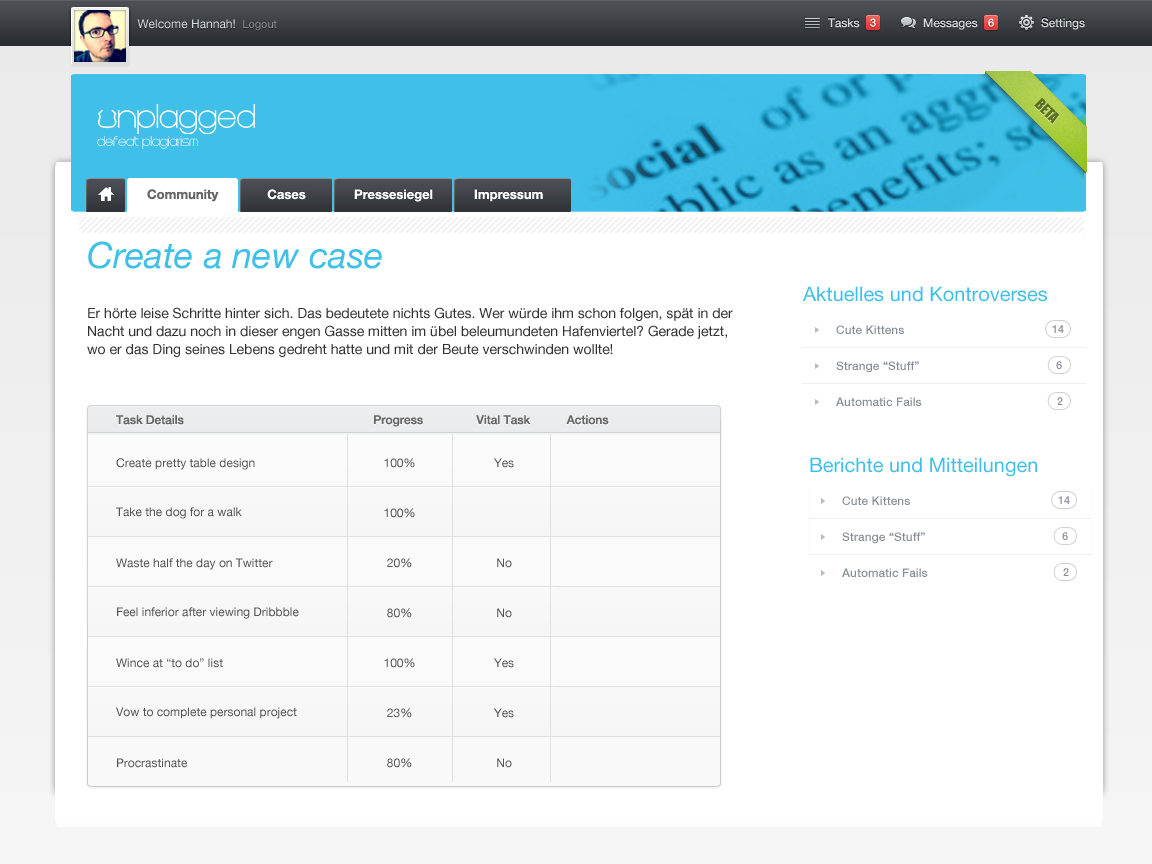
\includegraphics[width=0.97\textwidth]{images/init-psd.png}
  \caption{Initial Screen PSD}
  \label{fig:initialScreenPsd}
\end{figure}

The next step, before the HTML template got created, we defined the key features, our user interface should take care of:

\begin{itemize}
\item Reponsive Layout – optimized layouts for different devices
\item Cross-Browser-Compatibility
\item Light-weight and w3c-conform HTML5 Markup
\item Progressive enhcancement with CSS3 – CSS instead of images where possible
\end{itemize}

\subsection{Responsive Layout using CSS3 Media Queries}

Since the worldwide amount of different mobile and desktop devices is growing very fast, Ethan Marcotte coined the term
\textit{Resposive Webdesign}\citep{Marcotte2011} for websites that are not optimized for any devices at all, but  
simply for different screen resolutions. And this is what we do. 

Some functionality as uploading a file, doesn't work on iOS at 
all, but at least 
all functions that are working on mobile devices, should work. So the goal is to create a user interface that uses the 
same markup, but displays differently according to the device it is viewed on. Therefore CSS media queries are used, 
these are 
basically conditions that apply the CSS only if the condition is true. The most prominent conditions are 
the following:

\begingroup 
\begin{lstlisting}[caption=CSS Media Queries, label=list:cssMediaQueries, language=Ruby]
max-width: 600px  # max browser width 600px
min-width: 300px  # min browser width 300px
orientation:landscape # current orientation landscape mode
orientation:portrait # current orientation portrait mode
-webkit-min-device-pixel-ratio: 2 # min pixel ration (iPhone 4, Retina)
\end{lstlisting}
\endgroup

These media queries can be combined in any order to display an optimized page for each device. Since only the CSS 
changes, the HTML does not have to be touched. An example query looks like this: 

\begin{lstlisting}[caption=CSS Media Query, label=list:cssMediaQuery, language=Ruby]
@media only screen and (max-width: 600px) { }
\end{lstlisting}

Media queries are a CSS2 feature which most modern browsers, except IE9, implement. This isn't a problem though, because 
browsers that don't 
support them, just display the default css outside of the media queries, which is optimized for a width of about 1000 pixels 
in our case.

\subsection{Javascript and fallbacks}

Even though many websites require Javascript as mandatory for using the whole functionality range of the page, it is 
important to provide as much functionality as possible, when Javascript is turned of, to ensure accessibility\citep[page 323]{Zeldman2010}.
A short example will show how 
to implement a pagination with and without Javascript.

Usally when Javascript is disabled, the whole page will be reloaded, when the user changes to another page of the paginated content. The URL in this case will look something like this: \url{http://unplagged.local/document/list/page/2}. When Javascript is enabled, it is much faster to only refresh the area of the page, that really needs to reload, in this case the table with the content of the next page. It is only possible to change the hash of an URL, the part after the hash key (\#), using Javascript, the changed URL will be: \url{http://unplagged.local/document/list/#page/2}. An event called 'hashchange' can trigger a change of this part of the url and then reload the content through an AJAX request.

The pagination has the same HTML markup with and without Javascript, but with Javascript enabled it is much more convenient.

\begin{lstlisting}[caption=Javascript Pagination, label=list:cssMediaQuery, language=Ruby]
$(".pagination a").live("click", function() {
        var href = $(this).attr("href");
        if(href) {
          var substr = href.split('/');
          var hash = substr[substr.length-2] + "/" + substr[substr.length-1];

          window.location.hash = hash;
        }
        return false;
    });
    
    $(window).bind('hashchange', function(){
        var newHash = window.location.hash.substring(1);
        
        if (newHash) {
            var substr = newHash.split('/');
            var hash = substr[substr.length-2] + "/" + substr[substr.length-1];
            
            var url = window.location.pathname;
            if(url.charAt(url.length-1) != '/') {
              url += '/';
            }
            url += hash;
            $("#main-wrapper").load(url + " #main");
        };
        
    });
\end{lstlisting}


\section{Frameworks}
When we first discussed which programming language and frameworks, the Unplagged project should be built on, we figured 
out, that everyone was familiar with PHP. Since programming in a group requires a much better structure, than programming 
on your own, we needed a framework that requires a comfortable Model-View-Controller structure, we decided to use the Zend 
Framework. And to get rid of all the database issues as well as getting a flexibility in the used database system, we 
decided to use an Object-Relational-Mapping(ORM) framework, called Doctrine. What an ORM is, will be discussed later on.

\subsection{Zend Framework}
The Zend Framework is a typical PHP Framework using the Model-View-Controller pattern. Due to it's pre-defined directory 
structure, it is easy to get well seperated code. 

The directories and their meaning:
\begin{itemize}
\item application --- includes controller, models and view
\item data --- currently only includes i18n stuff (language stuff)
\item docs --- PHP Documentation and Developers Manual
\item library --- external and internal frameworks and extension to the Zend framework
\item public --- files that are accessible directly through the browser
\item scripts --- build scripts, deploying scripts
\item temp --- data that is overridden at any deployment
\item tests --- PHP Unit tests
\end{itemize}

The Zend framework offers RESTful\footnote{See for example \enquote{RESTful Web Services} of Richardson and Ruby for 
more information} URLs that follow a fixed pattern: \texttt{unplagged.local/controller/action/key/value/key2/value2}. Each 
controller is defined as ControllerNameController.php in the \texttt{application/controllers} directory and includes 
all possible actions. For example a file controller will look like this:

\begin{lstlisting}[caption=Persisting an object to the database in Doctrine, label=list:persistingObjectDoctrine, language=PHP]
class FileController extends Zend_Controller_Action{
	public function init(){
	}

	public function indexAction(){
	}

	public function uploadAction(){
	}

<<<<<<< HEAD
  public function listAction(){
=======
	public function listAction(){
>>>>>>> 7a2ccf18eebad5d280d777f496be384bdf2a24f8
	}
  	
	public function downloadAction(){
	}
}
\end{lstlisting}

By default, if no action is defined, the \texttt{indexAction} is called. For each action the appropriate view is by 
default rendered in the \texttt{application/views/scripts/conntrollerName/actionName.phtml} file.

The \texttt{models} directory includes all the objects, this will be discussed in more detail in the following chapter about Doctrine.

\subsection{Doctrine}
The whole database connection management of Unplagged is implemented using the Doctrine Framework in version 2. 
It consists of two layers, a database abstraction layer (DBAL) and an object relational mapping framework
(ORM). The DBAL uses PDO, a PHP framework for encapsulating database statements. The DBAL manages the
communication with any kind of SQL database and offers an own query syntax. This has the advantage, that
the database behind the framework can be changed from MySQL, to OracleSQL, PostgreSQL or SQLite at any time.
The DBAL is the agent between PDO and the ORM. The ORM is the connection between PHP objects and the DBAL.

Before the use of Doctrine is described, it will be explained, how the database on a new machine can be created 
and how the database structure can be updated, whenever something changed in the structure. Actually this is very easy, 
it is required to have a local MySQL database at this point having root' as a username, no password and a database 
called 'unplagged'. It is also possible to create a new configuration in the 
application/configs/application.ini file, although this step will not be described in this chapter. If the database is 
created, the build script can be executed:

\begin{lstlisting}[caption=Updating database structure, label=list:updatingDbStructure, language=Ruby]
php unplagged.local/scripts/build/doctrine.php
\end{lstlisting}

Now, the database is created or updated. If the database already existed, the data in it will not be removed! 
As described below, the big advantage of ORM is, that the programmer can stay in the PHP object context at any time. 
The only thing that has to be done additionally, is adding
comments to the member variables of a class, that define the fields in the database:

\begin{lstlisting}[caption=Defining a class in Doctrine, label=list:definingClassDoctrine, language=Ruby]
/** @Entity */
class UserClass
{
  /** @Column(type="integer") */
  private $id;
  /** @Column(length=30) */
  private $username;
}
\end{lstlisting}

The whole syntax documentation of doctrine can be found here: 

\begin{itemize}
\item \url{http://docs.doctrine-project.org/projects/doctrine-orm/en/latest/index.html} 
\end{itemize}

To persist a new object to the database, the persist method on this object has to be called, this writes the object 
into the doctrine cache. It stays in the cache, until the flush method is called, which actually executes all the 
previous operation since the last flush. These cann be deleting, updating, or editing an object.

\begin{lstlisting}[caption=Persisting an object to the database in Doctrine, label=list:persistingObjectDoctrine, language=Ruby]
$user = new User();
$user->setUsername('Max');
$em->persist($user);
$em->flush();
\end{lstlisting}

As the previous examples show, no database programming is necessary to create or persist a new object to the database, 
everyhting can be done in the PHP object context.
